\Section{Маршрутизация}{Лекции 4-5}{Игорь Смирнов}

Маршрутизация~--- функция сетевого уровня.

Это процесс доставки пакетов через сеть от одного узла до другого, когда эти узлы не соединены между собой непосредственно.

Маршрутизация бывает индивидуальной и групповой. Мы будем говорить только про индивидуальную.

Ключевая точка обмена трафиком в СПб~--- на Марсовом поле, в здании компании Ленэнерго.

\Subsection{Маршрутизаторы}

Это устройство сетевого уровня, реализующее функции маршрутизации (обеспечивающее доставку пакетов от одного узла сети к другим).

Другие названия маршрутизаторов:
\begin{MyItemize}
    \item Шлюз
    \item Router
    \item Gateway
\end{MyItemize}

Маршрутизатор отличается от конечного узла тем, что он пересылает входящие пакеты, у которых адрес назначения не совпадает с локальным адресом узла. Это называется {\bf IP-forwarding}.

Виды маршрутизаторов:
\begin{MyItemize}
    \item Аппаратные (маршрутизатор, router)
    \begin{MyItemize}
        \item Поддержка различных канальных сред
        \item Несколько сетевых интерфейсов
        \item Высокая производительность
        \item Высокая надёжность
        \item Хорошая защищённость
        \item Дополнительные функции: фильтрация, трансляция адресов, сбор статистики
        \item Обычно высокая стоимость
    \end{MyItemize}
    \item Программно-аппаратные (шлюз, gateway)
    \begin{MyItemize}
        \item Реализуются функциями ОС общего назначения
        \item Характеризуются невысокой производительностью, невысокой стоимостью
        \item Могут совмещать функции с обычными функциями ОС
    \end{MyItemize}
\end{MyItemize}

Процесс маршрутизации:

\begin{figure}[H]
  \centering
  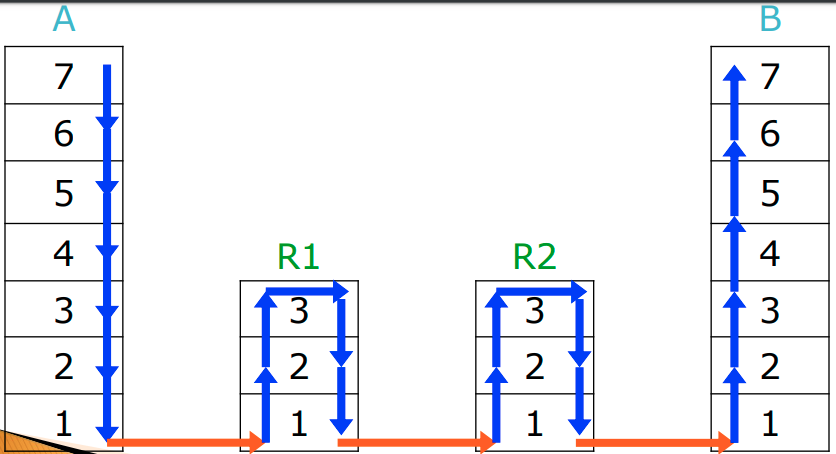
\includegraphics[width=15cm]{images/04/01}
\end{figure}

Маршрутизатор поднимает пакет до сетевого уровня. Если пакет предназначался не ему, посылает следующему маршрутизатору.

\Subsection{Виды маршрутизации}

\begin{MyItemize}
    \item По адаптивности:
    \begin{MyItemize}
        \item Статическая
        \item Динамическая
        \item <<От источника>>
    \end{MyItemize}
    \item По месту маршрутных вычислений:
    \begin{MyItemize}
        \item Централизованные
        \item Децентрализованные
    \end{MyItemize}
    \item По требуемой информации:
    \begin{MyItemize}
        \item Локальные
        \item Глобальные
        \item Смешанные
    \end{MyItemize}
\end{MyItemize}

(это всё уже было, поэтому пояснять не буду)

\Subsection{Таблицы маршрутизации}

О том, как они создаются, поговорим отдельно.

Таблицы маршрутизации состоят из:
\begin{MyItemize}
    \item Атрибутов маршрутных записей
    \begin{MyItemize}
        \item Сеть/узел назначения
        \item Сетевой интерфейс (через который нужно посылать на этот узел/сеть)
        \item Маршрутизатор (адрес)
        \item Метрика маршрута (стоимость маршрута)
        \item Флаги (каким образом маршрут был получен)
    \end{MyItemize}
    \item Псевдомаршрутов
    \begin{MyItemize}
        \item Дополнительные записи в таблице маршрутизации
        \item Используются для унификации процедуры поиска маршрута
        \item Бывают двух типов: на IP-адреса собственных сетевых интерфейсов и на подключённые IP-сети. Ни в одном, ни в другом случае реальная маршрутизация не нужна, поскольку доставка делается в рамках канальной сети. Но для унификации они добавлены в таблицу маршрутизации.
    \end{MyItemize}
\end{MyItemize}

Маршрут <<по умолчанию>>~--- маршрут, который выбирается, если ни одна из наших записей не подошла для входящей дейтаграммы.

Обозначается {\tt 0.0.0.0/0.0.0.0} (по сути это обозначение всей сети Internet). 

Управлять таблицей маршрутизации можно с помощью утилиты route.

Пример таблицы маршрутизации:

\begin{figure}[H]
  \centering
  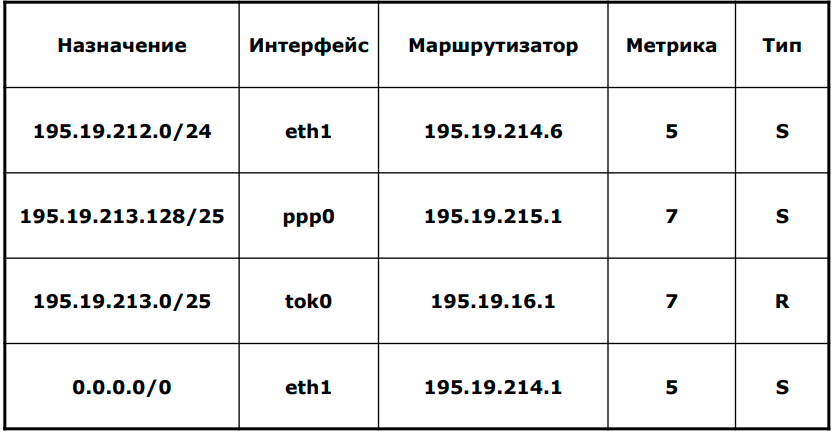
\includegraphics[width=15cm]{images/04/02}
\end{figure}

В классической маршрутизации адрес источника вообще не используется. Но, например, провайдерам это бывает нужно. Например, у нас есть дорогой клиент, который требует определённого уровня качества и есть дешёвый клиент, которому мы не гарантируем скорость доставки. Тогда дорогого клиента можно отправлять по <<чистому>> пути.

По умолчанию, TCP/IP поддерживает только одну таблицу маршрутизации. Но в некоторых системах поддерживается несколько таблиц маршрутизации.

В этих системах в зависимости от адреса источника выбирается подчинённая таблица маршрутизации, а в ней уже маршрутизация по адресу приёма.

Так можно решать задачу о балансировке трафика, например.

\Subsection{Статическая маршрутизация}

Все маршруты создаются вручную администратором, хранятся в таблицах до выключения.

\begin{figure}[H]
  \centering
  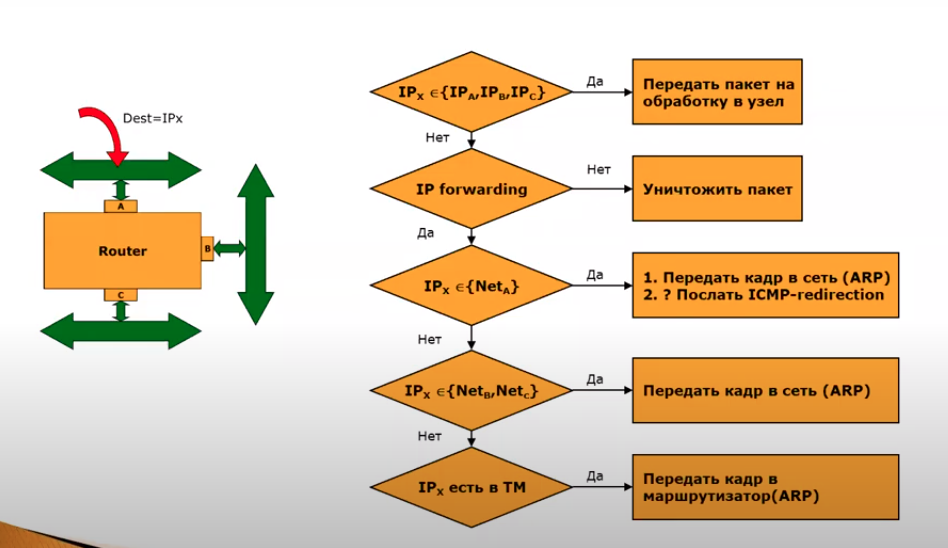
\includegraphics[width=15cm]{images/04/03}
\end{figure}

Псевдомаршруты помогают убрать 3 и 4 ромбики. Мы считаем, что это такие же адреса и маршрутизируем их по тому же правилу, что и 5. (оптимизации, которые мы заслужили)

\Subsection{Динамическая маршрутизация}

Статическая маршрутизация никак не зависит от ситуации в сети. Каналы связи могут обрываться, добавляться новые, маршрутизаторы могут выходить из строя...

{\bf Кулстори.} Основная причина сбоев интернета в России~--- экскаватор порвал волокно.

Что меняется в сети:
\begin{MyItemize}
    \item Топология
    \begin{MyItemize}
        \item Появление новых узлов
        \item Появление новых каналов
        \item ...
    \end{MyItemize}
    \item Каналы связи
    \begin{MyItemize}
        \item Выход из строя канала
        \item Ввод в строй канала
    \end{MyItemize}
    \item Узлы сети
    \begin{MyItemize}
        \item Выход из строя маршрутизатора
        \item Ввод в строй маршрутизатора
    \end{MyItemize}
    \item Нагрузка
\end{MyItemize}

\Subsection{Алгоритмы динамической маршрутизации}

Задача оптимальной маршрутизации~--- найти оптимальный путь для пакета в данный момент времени.

Поиск оптимального маршрута~--- поиск кратчайшего пути на графе.

Узлы графа~--- маршрутизаторы, дуги~--- каналы, веса~--- метрика.

Под оптимальностью можно понимать разные вещи:
\begin{MyItemize}
    \item Минимальное время доставки
    \item Минимальная стоимость доставки
    \item Минимальная задержка
    \item ...
\end{MyItemize}

Из алгоритмов используют Форда-Беллмана и Дейкстру и их модификации.

Расписывать ФБ и Дейкстру не буду.

ФБ работает за $\O(V^3)$ (это, конечно, правда, но аааааааа, $\O(VE)$ же... Или сеть~--- это почти полный граф?), но у нас ФБ с break, поэтому он работает более-менее норм. А ещё он легко параллелится.

Это локальный алгоритм (то есть нам не нужно знать топологию всей сети (а почему это так~--- увидим позже)).

{\bf Кулстори.} Дейкстра получил премию имени Дейкстры. Он создал эту премию, умер, премию переименовали в его честь и дали ему посмертно.

Время работы Дейкстры $\O(V^2)$.

Тут, в отличие от ФБ, нам нужно знать топологию всей сети. А ещё Дейкстра не очень хорошо параллелится.

Дейкстра требует $\O(V^2)$ памяти <<на хранение всей матрицы расстояний>> и это проблема при больших $V$ (тут был пример про $V\approx 10\,000$, но блин, ну правда же, что граф такой сети обычно прямо совсем не полный?..) 

\Subsection{Системы маршрутизации}

AS~--- автономная система.

Имеет уникальный номер.

AS:
\begin{MyItemize}
    \item Часть сети, управляющаяся из одного центра управления
    \item Реализующая одну политику маршрутизации
    \item Внутри AS обеспечиваются одинаковые протоколы маршрутизации
\end{MyItemize}

То есть это такой локальный центр управления маршрутизацией в интернете.

\begin{figure}[H]
  \centering
  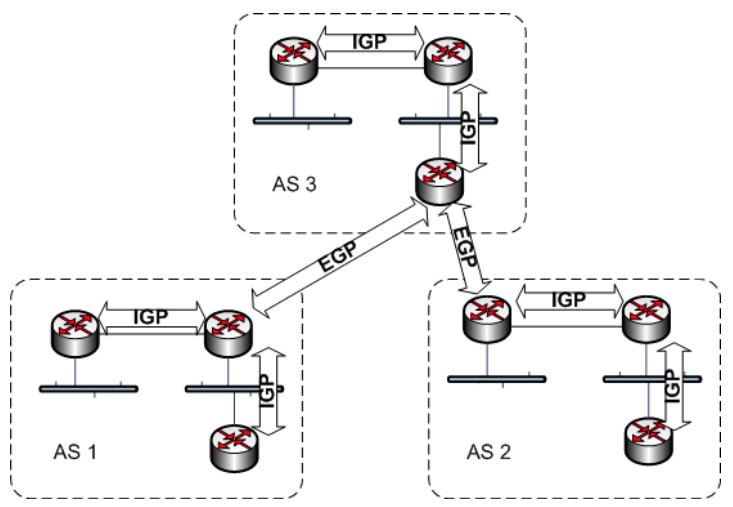
\includegraphics[width=15cm]{images/04/04}
\end{figure}

Протоколы маршрутизации внутри AS~--- внутренние (IGP~--- Interior Gateway Protocol), между AS~--- внешние (EGP~--- Exterior Gateway Protocol).

Некоторые маршрутизаторы являются пограничными и обеспечивают связь между разными AS.

\Subsubsection{Протоколы маршрутизации}

Характеристики:
\begin{MyItemize}
    \item Название 
    \item Стандартизирующие документы
    \item Алгоритм поиска маршрута
    \item Метрика протокола
    \item Сходимость~--- способность протокола оперативно реагировать на изменения в сети и приводить маршрутизаторы к соответствующее состояние\\
    Время сходимости – время за которое маршрутные таблицы переходят в состояние, адекватное изменившейся ситуации сети
    \item Избежание петель маршрутизации
    \item Загрузка сети
    \item Ресурсоёмкость
    \item Поддержка нескольких маршрутов на сеть (однопутевые или многопутевые)
    \item Аутентификации
    \item Ограничения применения
    \item Конфигурирование
    \item Поддержка в маршрутизаторах
\end{MyItemize}

\Subsubsection{Метрики маршрутов}

Метрика может зависеть от:
\begin{MyItemize}
    \item Числа промежуточных маршрутизаторов
    \item Пропускной способности канала связи
    \item Задержек в канале связи
    \item Надежности канала связи
    \item Загрузки канала связи
\end{MyItemize}

В общем случае, метрика моет быть комбинацией этих параметров.

\Subsection{Внутренние протоколы маршрутизации}

\begin{MyItemize}
    \item RIP
    \item OSPF
    \item IGRP
    \item EIGRP
    \item IS-IS
    \item ...
\end{MyItemize}

\Subsubsection{Протокол маршрутизации RIP}

Routing Information Protocol

Используется в TCP/IP и Novell

Использует ФБ.

Тип протокола~--- однопутевой. То есть может хранить только один путь на целевую сеть.

Самая слабая его сторона~--- метрика. В нём это целое число от 0 до 15, которое означает число промежуточных маршрутизаторов до сети назначения. Для соседей~--- 0, 16~--- сеть недоступна.

Эта метрика не зависит от задержек, пропускной способности, надёжности, загрузки.

Граф для ФБ~--- с единичными весами рёбер.

Алгоритм функционирования RIP:
\begin{enumerate}
    \item Рассылка соседям маршрутной информации (по сути рассылаем соседям свою таблицу маршрутизации со своими текущими расстояниями). Это происходит раз в 30 секунд
    \item Корректировка собственной ТМ после получения обновления от соседей (по сути тоже получаем их таблицы маршрутизации с текущими расстояниями)
\end{enumerate}

{\bf Корректировка таблицы:}

\begin{figure}[H]
  \centering
  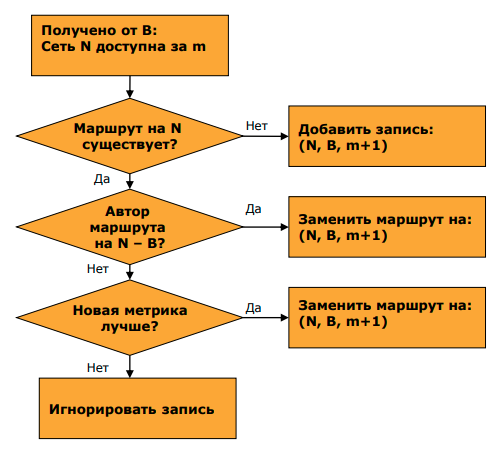
\includegraphics[width=15cm]{images/04/05}
\end{figure}

При корректировке, если к нам прислали новый маршрут, мы должны не просто сделать {\tt min=}.

Допустим, узел B говорит, что сеть N доступна за m шагов. Если наш путь на N проходил через B, то мы в любом случае должны обновить расстояние, даже если оно стало хуже, потому что B лучше знать, какой путь до N (мало ли там что-то испортилось).

При этом мы на каждый маршрут в таблице заводим таймер. Если больше трёх минут сосед нам ничего не посылает, то мы по прежнему используем его для маршрутизации, но уже не рассылаем соседям.

А если сосед нам ничего не посылает больше 5 минут, то мы удаляем этот маршрут из нашей таблицы маршрутизации.

{\bf Петли маршрутизации}

Пусть сеть A подключена к сети B, а та непосредственно подключена к сети N.

И вдруг внезапно кабель до сети N порвался и она перестала быть доступна. Тогда обновляться таблицы маршрутизации будут как показано на картинке:

\begin{figure}[H]
  \centering
  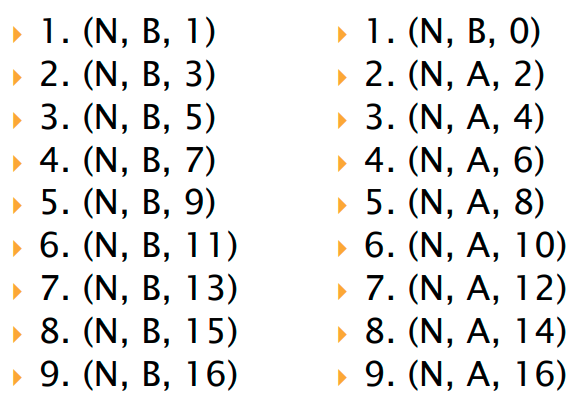
\includegraphics[width=15cm]{images/04/06}
\end{figure}

И только на 9 шаге мы поймём, что сеть N недоступна. То есть мы только через 5 минут узнаем об этом. А всё это время пакеты будут гоняться между A и B и умирать по TTL. Это, к тому же, загружает сеть. Печально.

Чтобы бороться со всем этим, придумали несколько технологий преодоления петель маршрутизации. {\it А что самое главное в технологии преодоления? Хорошее название.}
\begin{MyItemize}
    \item Split Horizon~--- расщепление горизонта.\\
    Обновления не посылаются на тот интерфейс, из которого этот маршрут получен. 
    \item Poison Reverse~--- обратный яд\\
    Обновления маршрута посылаются на интерфейс, из которого этот маршрут получен, но с метрикой 16
    \item Triggered Updates~--- мгновенные обновления\\
    Если в сети происходит какое-то изменение, то забываем про 30-секундные интервалы и начинаем сразу передавать информацию.\\
    Ускоряется сходимость протокола, но при этом лавинообразно увеличивается трафик.
    \item Hold Down\\
    Кратковременное прекращение приема обновлений маршрута после получения его обновления от автора с метрикой 16\\
    В течение 120 с маршрутизатор не принимает обновления этого маршрута, пережидая переходные процессы в сети\\
    {\it <<Когда мы кидаем камни в воду, некоторое время круги расходятся. Идея Hold Down: давайте переждём эти переходные процессы в сети>>}
\end{MyItemize}

На практике используют сразу несколько из этих технологий. 

{\bf Никакие технологии не спасают от петли маршрутизации, включающей более 2 узлов.}

{\bf Транспортировка данных в RIP.}

Соседние маршрутизаторы~--- широковещательно.

Рассылка обновлений: {\tt 255.255.255.255} (все узлы данной локальной сети).

RIP инкапсулируется в UDP (порт 520).

В один пакет входит до 25 маршрутных записей. Максимальная длина пакета~--- 512 байт.

Формат пакета:

\begin{figure}[H]
  \centering
  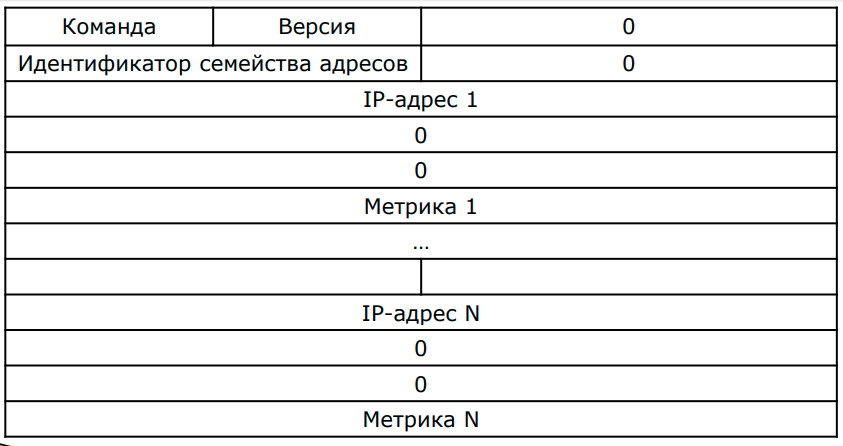
\includegraphics[width=15cm]{images/04/07}
\end{figure}

\begin{MyItemize}
    \item Команда~--- код операции (1~--- запрос, 2~--- ответ)\\
    Запрос нужен, если у нас появилась новая станция. Она не ждёт 30 секунд, а сразу посылает запрос, чтобы ей скинули таблицы маршрутизации.
    \item Идентификатор семейства адресов~--- тип сетевой среды (для TCP/IP~--- 2)
    \item IP-адрес~--- адрес сети класса A, B или C. То есть RIP не поддерживает подсети.
\end{MyItemize}

Итого: RIP~--- простой протокол, у него низкие требования к вычислительным ресурсам и объёмам памяти, легко настраивается (работает из коробки, но можно указать алгоритмы обхода петель и интерфейсы).

Но при этом плохая метрика, высокая нагрузка сети, ограниченный диаметр сети (15), медленная сходимость, не поддерживает маски подсети, нет подтверждения подлинности и шифрования.

{\bf Кулстори.} В 95 году на кафедре Политеха только появились компьютерные сети. И стала происходить странная ситуация: каждый четверг в 12:00 интернет отключался и переставал работать. А в 13:40 всё включалось и продолжало работать. Проблема была в следующем: на одном из кафедральных маршрутизаторов, подключённых к общей сети, был некорректно настроен сервис маршрутизации. Когда этот компьютер включали, он сообщал всем, что у него есть маршрут на сеть {\tt 0.0.0.0} с метрикой 0. Все перестраивали путь на него. А почему это происходило раз в неделю? Потому что интернет тогда был по расписанию, преподаватель в 12:00 приходил на работу, включал сервер, полтора часа вёл занятия и выключал его.

\Subsubsection{протокол маршрутизации RIP-II}

Появилась аутентификация, маска сети, групповая адресация вместо широковещательной, добавились метки маршрута и ссылка на следующий маршрутизатор.

Групповая адресация (по {\tt 224.0.0.9}) лучше широковещательной тем, что в широковещательной этот пакет получат все узлы, а тут только маршрутизаторы, использующие RIP.

Формат пакета:

\begin{figure}[H]
  \centering
  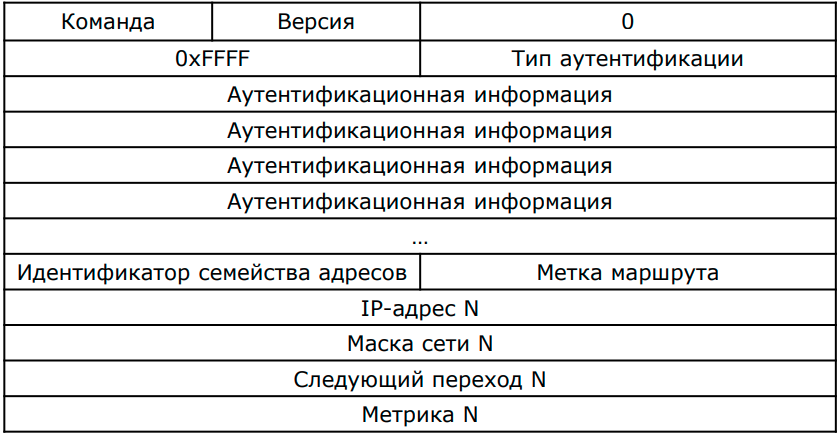
\includegraphics[width=15cm]{images/04/08}
\end{figure}

<<Следующий переход>> нужен для исключения лишних шагов в маршрутизации и для возможности использовать информацию из других источников (не из RIP-а).

Метка маршрута нужна для упрощения взаимодействия с EGP.

Совместим с RIP-1.

\Subsubsection{Протокол маршрутизации OSPF}

OSPF = Open Shortest Path First

Использует алгоритм Дейкстры.

Сейчас он очень широко используется.

Метрика~--- число от 0 до 65535~--- количество секунд, требуемое для передачи 100 Мбит через физическую среду данной сети
\begin{MyItemize}
    \item 10Base-T Ethernet – 10
    \item 56 кбит/с – 1785
    \item Метрика канала со скоростью передачи данных 100 Мбит/с и выше – 1
\end{MyItemize}

Для каждого канала связи метрика может задаваться администратором (если вдруг захотим трактовать метрику по-другому. Например, сейчас большинство сетей быстрее 100 Мбит/с).

Так как используется Дейкстра, мы должны всем узлам сообщить топологию. Для этого рассылаем пакеты LSA~--- Link State Advertisment. Там есть информация о каналах и их состояниях (метриках).

По сути каждый узел графа рассказывает о своих дугах.

Рассылка осуществляется только если что-то меняется. 

Рассылаются лавинным образом (то есть все шлют одновременно) и все получают информацию о всех.

Все маршрутизаторы строят LSD~--- Link State Database. Чтобы протокол работал корректно, нужно чтобы все LSD были одинаковыми.

На основе LSD строим LST~--- Link State Tree (просто дерево Дейкстры из этой вершины).


Причины рассылки LSA:
\begin{MyItemize}
    \item Изменилось состояние интерфейса
    \item Произошли изменения в маршрутизаторе сети
    \item Произошло изменение состояния одного из соседних маршрутизаторов
    \item Изменилось состояние одного из внутренних маршрутов
    \item Изменение состояния межзонного маршрута
    \item Появление нового маршрутизатора, подключенного к сети
    \item Возникли изменения одного из внешних маршрутов
    \item Маршрутизатор перестал быть пограничным для данной AS (например, перезагрузился)
    \item Возраст маршрута достиг предельного значения (30 минут)
    \item ...
\end{MyItemize}

{\bf Таблица маршрутизации OSPF}
\begin{MyItemize}
    \item IP-адрес места назначения и маска
    \item Тип места назначения (сеть, граничный маршрутизатор и т.д.)
    \item Тип сервиса (TOS)~--- OSPF позволяет строить разные типы маршрутов для разных типов сервиса. 
    \item Домен маршрутизации
    \item Тип пути (внутренний; межобластной; внешний, ведущий к AS)
    \item Метрика
    \item Следующий маршрутизатор
    \item Объявляющий маршрутизатор (используется для межобластных обменов и для связей автономных систем друг с другом)
\end{MyItemize}

Не хочется грузить сеть лавинным трафиком. Давайте найдём в сети какой-нибудь маршрутизатор, все отправим ему, а уже он перешлёт всем. Это делают назначенные маршрутизаторы (DR~--- Designated Router).

Если он есть, то шлют LSA ему.

На всякий случай есть запасной~--- BDR (Backup Designated Router).

OSPF инкапсулируется в IP (с кодом 89).

Для передачи маршрутных обновлений используются адреса:
\begin{MyItemize}
    \item Для адресации всех OSPF-маршрутизаторов: {\tt 224.0.0.5}
    \item Для адресации всех назначенных OSPF-маршрутизаторов: {\tt 224.0.0.6}
\end{MyItemize}

В OSPF есть политика доменов маршрутизации. Если у нас есть большая сеть, то давайте разделим её на 4 подсегмента (например, мы можем захотеть это сделать, если у нас граф сети очень большой).

Внутри доменов своя маршрутизация, есть междоменная маршрутизация. 

Достоинства OSPF:
\begin{MyItemize}
    \item Гибкая метрика
    \item Быстрая сходимость (почти мгновенная)
    \item Низкая загрузка каналов служебным трафиком
    \item Отсутствие петель маршрутизации
    \item Поддержка доменов маршрутизации (позволяет уменьшить требования к ресурсам сети)
    \item Поддержка различных маршрутов для разных типов обслуживания (он такой единственный из тех, что мы рассмотрим. Если нужна сеть с TOS, то, это, пожалуй, единственный вариант)
\end{MyItemize}
Недостатки OSPF:
\begin{MyItemize}
    \item Высокие требования к ресурсам:
    \begin{MyItemize}
        \item Быстродействие
        \item Объемы памяти для хранения LSD, LST
    \end{MyItemize}
    \item Высокая сложность конфигурирования (надо конфигурировать идентификатор домена маршрутизации, все параметры каналов связи для каждого маршрутизатора)
\end{MyItemize}

\Subsubsection{Протокол маршрутизации EIGRP}

Это расширение IGRP. Но IGRP не рассматриваем, потому что он устаревший.

Enhanced Interior Gateway Routing Protocol.

Разработан компанией Cisco и не регламентируется RFC (это редкость).

IGRP~--- это был продвинутый RIP, но он проигрывал OSPF.

Это гибридный протокол. Он дистанционно-векторный с элементами протокола состояния канала.

Основные особенности:
\begin{MyItemize}
    \item Механизм обнаружения соседей
    \item Посылка обновлений таблиц
    \item Вычисление вероятных заместителей (механизм запасных маршрутов)
    \item Алгоритм активного поиска DUAL (на случай плохого состояния в сети)
\end{MyItemize}

Метрика~--- самая сильная часть этого протокола.

Определяется параметрами:
\begin{MyItemize}
    \item Задержка (D~---Internwork delay)~--- значение в диапазоне 10 мкс~-- 167 с
    \item Ширина полосы (B~---bandwidth)~--- значение в диапазоне 1200 б/с~-- 10Гб/с (для текущих сетей {\it почти} подходит. Сейчас у самых быстрых промышленных сетей 100Гб/с)
    \item Надежность (R~---reliability)~--- определяется вероятностью успешной посылки в данном канале связи (0-1). Можно вычислять по статистике.
    \item Нагрузка (L~---load)~--- определяется долей занятости канала (0-1)
\end{MyItemize}

$M=(K_1\cdot B + \frac{K_2\cdot B}{256-L} + K_3\cdot D)\cdot\frac{K_5}{R+K_4}$ при $K_5\neq 0$

$M=K_1\cdot B + \frac{K_2\cdot B}{256-L} + K_3\cdot D$ при $K_5= 0$

Коэффициенты $K_{1..5}$ определяются пользователем

По умолчанию:

$K_1=K_3=1$

$K_2=K_4=K_5=0$

$M=B+D$

Задержка измеряется в 10 мкс. $D\in[1..2^{24}]$

Полоса пропускания~--- в Кбит/с. $B\in[1..2^{24}]$

Надёжность~--- доля успешно переданных и принятых пакетов. $R\in[0..255]$

Загрузка~--- занятая часть канала в процентном соотношении. $L\in[0..255]$

{\bf Механизм обнаружения соседей.}

Хотим получать информацию о соседях маршрутизатора. Для этого посылается пакет {\tt Hello} (для быстрых сетей раз в 5 секунд, для медленных раз в 60 секунд).

По получаемым сообщениям делаем выводы об имеющихся соседях (например, можем сохранять все полученные пакеты и смотреть, когда нам в последний раз с определённого IP-адреса что-то отправляли).

{\bf Таблица топологии.}

Вместо таблицы маршрутизации тут используют таблицу топологии. Она расширяет таблицу маршрутизации.

Она предназначена для выбора маршрутов на сеть назначения.

Поля:
\begin{MyItemize}
    \item Минимальная полоса пропускания в пути
    \item Общая задержка пути
    \item Надежность пути
    \item Загрузка пути\\
    Эти 4 параметра рассчитаны по всему каналу связи.
    \item Минимум MTU на пути
    \item Текущая дистанция~--- текущее значение метрики сети маршрута от нашего узла до сети назначения
    \item Отчетная дистанция~--- та дистанция, которую нам прислал источник, до того, как мы её увеличили на $d$ нашего канала (то есть путь без одного ребра)
    \item Источник маршрута
\end{MyItemize}

{\bf Выбор путей.}

Когда хотим определить оптимальный маршрут, мы выбираем путь с наименьшей дистанцией.

Также выбираются запасные пути~--- вероятные заместители. Они выбираются так, чтобы отчётная дистанция была меньше текущей дистанции оптимального маршрута.

\begin{figure}[H]
  \centering
  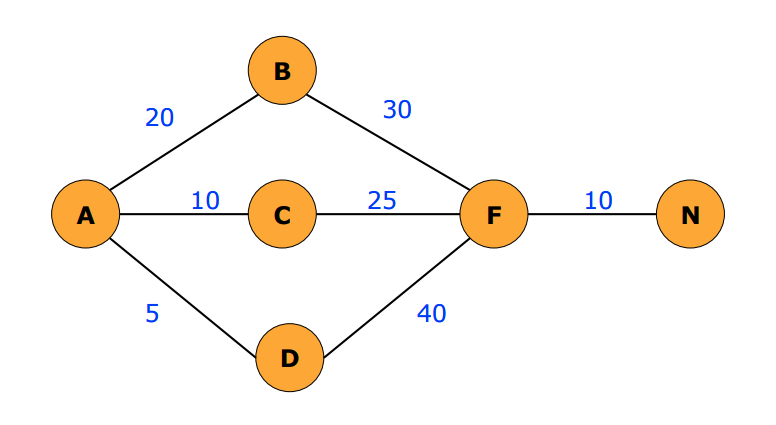
\includegraphics[width=15cm]{images/04/09}
\end{figure}

На этом примере оптимальный маршрут~--- ACF (с длиной 45).

А заместителем будет маршрут через B (потому что его отчётная дистанция~--- 40, тогда как отчётная дистанция маршрута через D~--- 50, хоть маршрут через D и короче).

Это сделано так, чтобы избежать петель маршрутизации. Посмотрим на мир глазами маршрутизатора A. Он видит только соседей и расстояния от них до N. И возможно такое, что оптимальный маршрут через D проходит обратно через A, а дальше по оптимальному маршруту для A. Тогда если оптимальный маршрут для A сломается, сломается и этот маршрут. А наше правило (отчётная длина меньше длины оптимального) гарантирует нам, что такого не случится. 

{\bf Алгоритм DUAL.}

Diffuse Update Algorithm.

Используется для активного поиска маршрута в случает удаления его из таблицы маршрутизации.

\begin{MyItemize}
    \item Станция, потерявшая маршрут, использует вероятного заместителя
    \item Если его нет - посылает запрос соседям
    \item Если сосед имеет вероятного заместителя~--- посылает ответ
    \item Если сосед не имеет~--- сам начинает процедуру активного поиска (для поиска использует все интерфейсы, кроме входящего)
\end{MyItemize}

{\bf Типы пакетов в EIGRP.}

\begin{MyItemize}
    \item Приветствие (Hello)
    \begin{MyItemize}
        \item Используется для группового оповещения соседей
        \item Не требует подтверждения
    \end{MyItemize}
    \item Обновление (Update)
    \begin{MyItemize}
        \item Если обнаружен новый сосед~--- обновление посылается индивидуально
        \item Если изменение в маршруте~--- обновление посылается по групповому адресу
    \end{MyItemize}
    \item Запрос (Query)~--- для DUAL
    \begin{MyItemize}
        \item Запросы по групповому адресу
    \end{MyItemize}
    \item Ответ (Reply)~--- для DUAL
    \begin{MyItemize}
        \item Посылаются в ответ на запрос
        \item Сообщают автору, что есть вероятный заместитель
        \item Всегда отправляются индивидуально автору запроса
    \end{MyItemize}
    \item Запрос информации (Request)
\end{MyItemize}

Метрики каналов <<по умолчанию>>:

\begin{figure}[H]
  \centering
  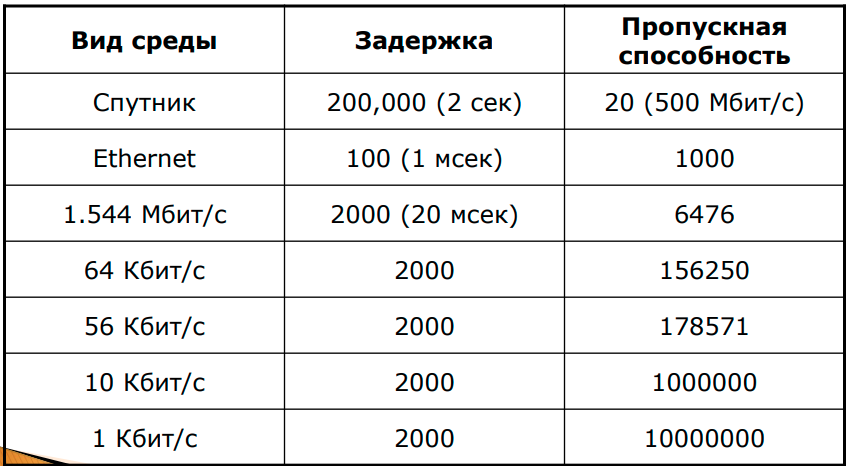
\includegraphics[width=15cm]{images/04/10}
\end{figure}

Это всё можно перенастроить.

В качестве транспорта в EIGRP используется IP (номер 9).

А ещё Cisco зачем-то получила номер 88 в IP для IGRP/EIGRP, но не использует его.

Используется широковещательный механизм рассылки маршрутных обновлений.

Достоинства EIGRP:
\begin{MyItemize}
    \item Очень малое использование сети в нормальном состоянии (только передача Hello)
    \item При изменениях посылаются только изменения маршрутных таблиц
    \item Низкое время сходимости
    \item Обход петель маршрутизации
    \item Поддержка маски сети
    \item Простота реализации
\end{MyItemize}

Недостатки EIGRP:
\begin{MyItemize}
    \item Несколько худшая по сравнению с OSPF сходимость
\end{MyItemize}

\Subsection{Протоколы внешней маршрутизации}

Нужны чтобы передавать пакеты между AS.

Всего таких протоколов два: EGP и BGP.

\Subsubsection{EGP}

External Gateway Protocol

Не имеет метрики (по сути протокол достижимости).

Единицей измерения была не одна сеть или один IP-адрес, а целая автономная система.

Сейчас уже почти не используется.

\Subsubsection{BGP}

Основан на Дейкстре.

Текущая версия~--- 4.

Используется для междоменной маршрутизации.

Оперирует тоже автономными системами.

Как транспорт использует TCP (порт 179). Это единственный протокол маршрутизации, использующий TCP.

В жизни мы его встретим максимум в одном случае~--- если будем работать у провайдеров первого уровня.

Вообще, ещё есть протокол ES-IS, но он вообще не используется.

